%\documentclass[a4paper, 12pt]{report}

%\usepackage[utf8]{inputenc}

% Logos
\newcommand{\ulb}{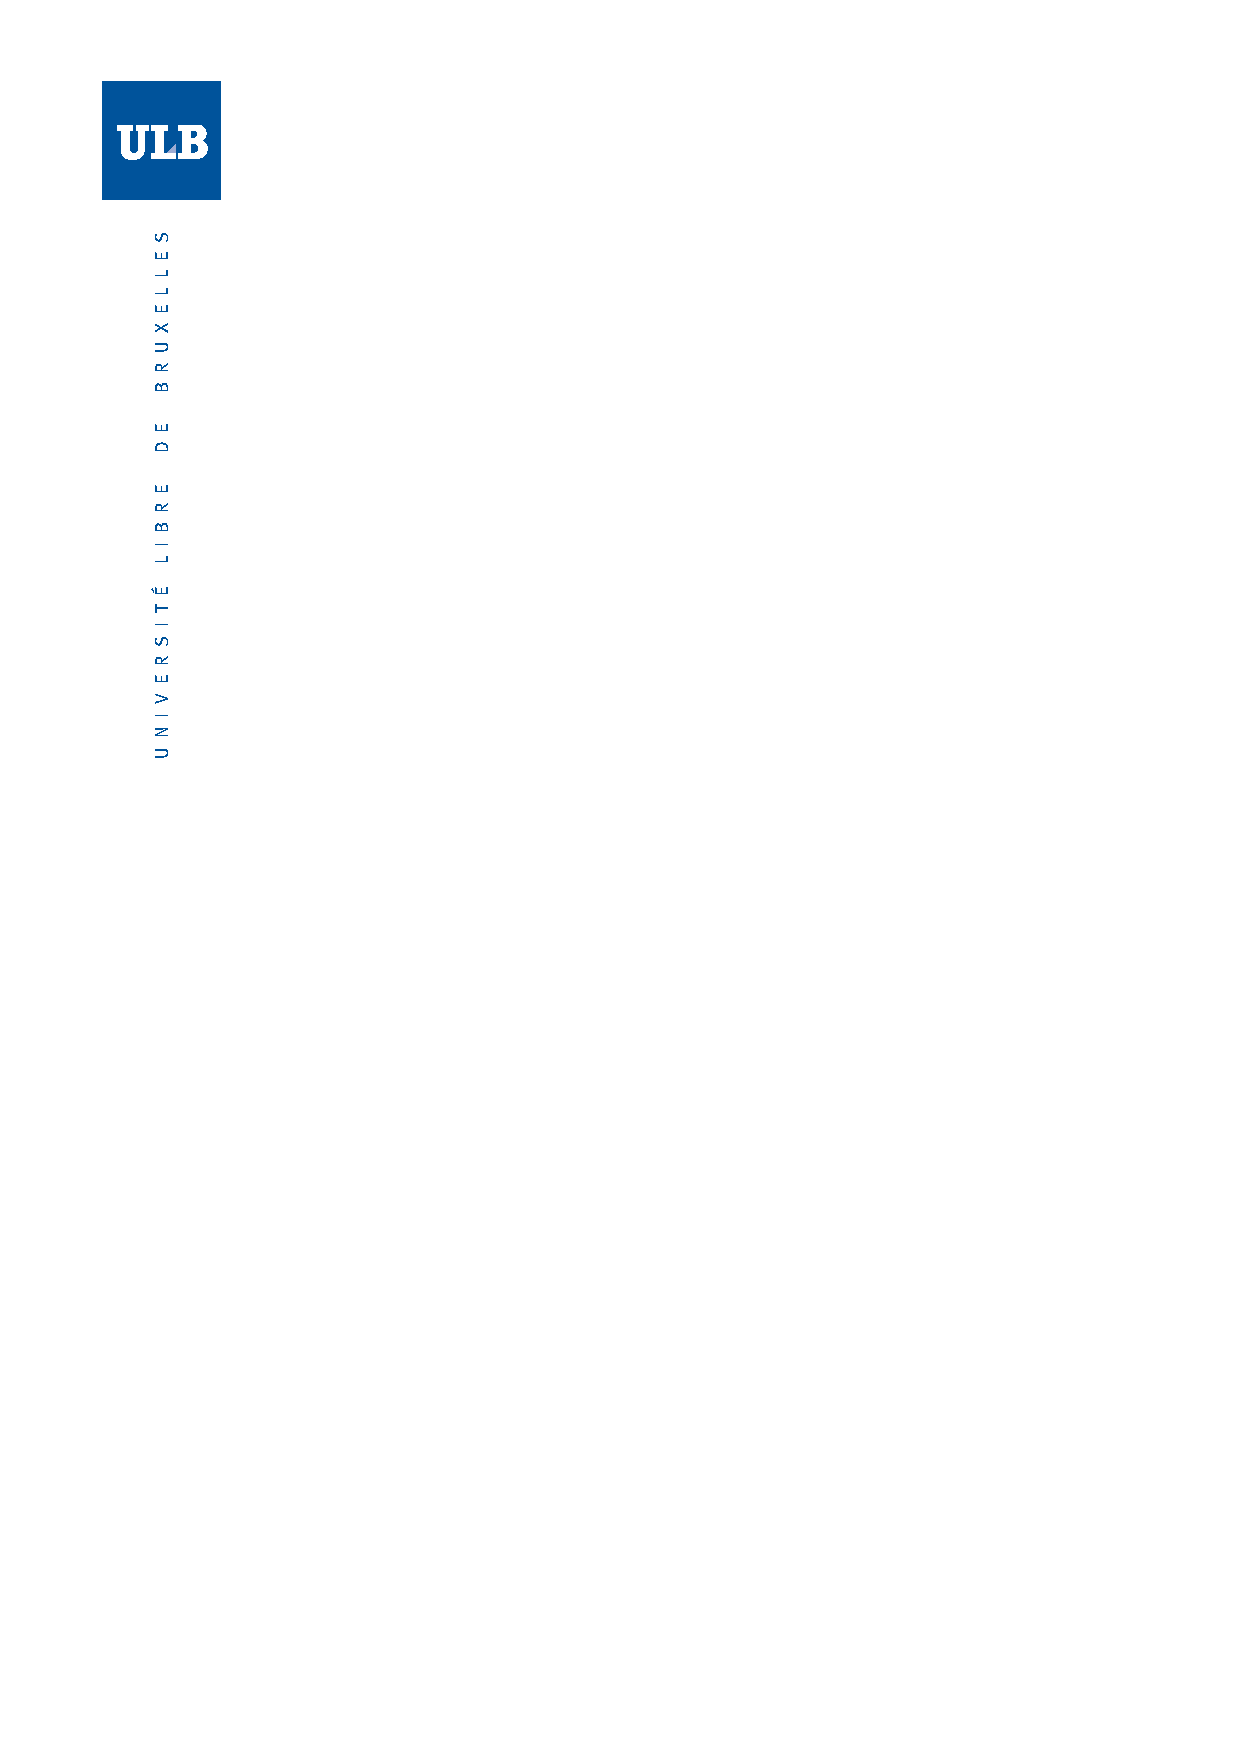
\includegraphics[scale=1.1]{images/logo_ULB2.pdf}}
\newcommand{\polytech}{
\includegraphics[scale=0.35]{images/logo_polytech_FR.pdf}}

% Polices
\definecolor{ULBblue}{rgb}{0,0.2196,0.5765}
\newcommand{\fontTitle}{\sffamily \Huge\selectfont \color{ULBblue}}
\newcommand{\fontSubtitle}{\sffamily \LARGE \selectfont \color{ULBblue}}
\newcommand{\fontText}{\sffamily \selectfont}
\newcommand{\fontColor}{\sffamily \selectfont \color{ULBblue}}

% Titre
\newcommand{\titleA}{\fontTitle{Majorization Lattice in the Theory of}} % Titre identique au titre remis au secrétariat
\newcommand{\titleB}{\fontTitle{Entanglement}} % (dans la langue de rédaction a priori)
% Sous-titre
\newcommand{\subtitle}{\fontSubtitle{}}
% Titre du diplôme
\newcommand{\diplomaA}{\fontText{Mémoire présenté en vue de l’obtention du diplôme}} % A laisser en Français
\newcommand{\diplomaB}{\fontText{d'Ingénieur Civil Physicien à finalité spécialisée}}

% Etudiant
\newcommand{\student}{\textbf{\sffamily \large Alexander Stévins}}

% Supervision
\newcommand{\promAa}{\fontColor{Directeur}}
\newcommand{\promAb}{\fontText{Professeur Nicolas Cerf}}
\newcommand{\promBa}{\fontColor{Co-Promoteur}}
\newcommand{\promBb}{\fontText{Professeur [Prénom Nom]}}
\newcommand{\promCa}{\fontColor{Superviseur}}
\newcommand{\promCb}{\fontText{Serge Deside}}
\newcommand{\deptA}{\fontColor{Service}}
\newcommand{\deptB}{\fontText{QuIC}}

% Année académique
\newcommand{\yearA}{\fontColor{Année académique}}
\newcommand{\yearB}{\fontText{2024 - 2025}}

%\begin{document}

	\thispagestyle{empty}
	\newgeometry{top=2.5cm, bottom=1.5cm, left=2.5cm, right=1cm}
	\setlength{\unitlength}{1mm}
	\noindent\begin{picture}(175,257)
	
		\put(0,245){\polytech}
		\put(153,139.5){\ulb}
		
		\put(8,150){\makebox(150,10)[l]{\titleA}}
		\put(8,140){\makebox(150,10)[l]{\titleB}}
		%\put(8,135){\makebox(150,10)[l]{\subtitle}}
		
		\put(0,75){
		\begin{tikzpicture}[scale=0.1]
		\fill [fill=ULBblue](0,0) rectangle (0.8,90);
		\fill [fill=ULBblue](0,57) rectangle (152,57.8);
		\end{tikzpicture}}
		
		\put(8,120){\makebox(150,5)[l]{\diplomaA}}
		\put(8,115){\makebox(150,5)[l]{\diplomaB}}
		
		\put(8,75){\makebox(150,10)[l]{\selectfont \student}}
		
		\put(8,31){\makebox(80,5)[l]{\promAa}}
		\put(8,26){\makebox(80,5)[l]{\promAb}}
		%\put(8,31){\makebox(80,5)[l]{\promBa}} % Commenter la ligne si pas nécessaire
		%\put(8,26){\makebox(80,5)[l]{\promBb}} % Commenter la ligne si pas nécessaire
		\put(8,18){\makebox(80,5)[l]{\promCa}} % Commenter la ligne si pas nécessaire
		\put(8,13){\makebox(80,5)[l]{\promCb}} % Commenter la ligne si pas nécessaire
		\put(8,5){\makebox(80,5)[l]{\deptA}}
		\put(8,0){\makebox(80,5)[l]{\deptB}}
		
		\put(145,5){\makebox(30,5)[r]{\yearA}}
		\put(145,0){\makebox(30,5)[r]{\yearB}}
	
	\end{picture}
	\restoregeometry

%\end{document}

% Template conçu par Benjamin Vanhemelryck et revu par François Bronchart - Mai 2013